%& C:\Users\tn5093\AppData\Roaming\TikzEdt\TikzEdt\023~1.0\TEMP_H~1
\begin{document}
\usetikzlibrary{arrows}
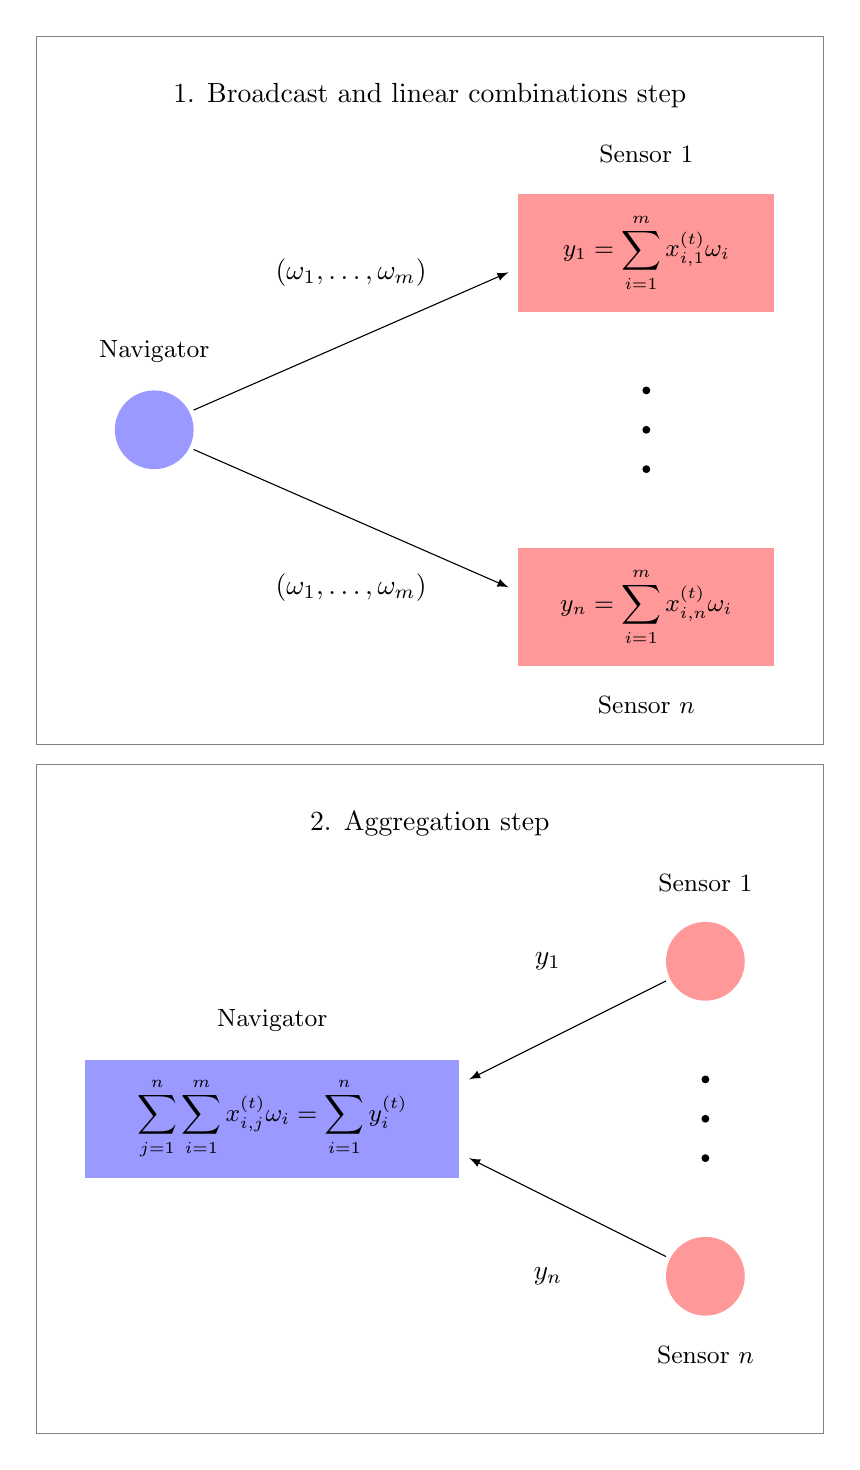
\begin{tikzpicture}
    % Step 1
    \node at (5,22.5) {1. Broadcast and linear combinations step};
    % Navigator
    \node at (1.5,19.25) {\small Navigator};
    \fill (1.5,18.25) [fill=blue!40] ellipse (0.5 and 0.5);
    % Sensors
    \node at (7.75,21.75) {\small Sensor $1$};
    \fill [fill=red!40] (6.125,19.75) rectangle (9.375,21.25);
    \node at (7.75,20.5) {\small $\displaystyle y_1 = \sum^m_{i=1}x_{i,1}^{(t)}\omega_i$};
    \node at (7.75,14.75) {\small Sensor $n$};
    \fill [fill=red!40] (6.125,15.25) rectangle (9.375,16.75);
    \node at (7.75,16) {\small $\displaystyle y_n = \sum^m_{i=1}x_{i,n}^{(t)}\omega_i$};
    \fill [black] (7.75,18.75) circle (0.05);
    \fill [black] (7.75,17.75) circle (0.05);
    \fill [black] (7.75,18.25) circle (0.05);
    % Lines
    \draw [-latex] plot[smooth, tension=.7] coordinates {(2,18.5) (6,20.25)};
    \draw [-latex] plot[smooth, tension=.7] coordinates {(2,18) (6,16.25)};
    \node at (4,20.25) {$(\omega_1,\dots ,\omega_m)$};
    \node at (4,16.25) {$(\omega_1,\dots ,\omega_m)$};
    
    % Step 2
    \node at (5,13.25) {2. Aggregation step};
    % Navigator
    \node at (3,10.75) {\small Navigator};
    \fill [fill=blue!40] (0.625,8.75) rectangle (5.375,10.25);
    \node at (3,9.5) {\small $\displaystyle \sum^{n}_{j=1}\sum^{m}_{i=1} x_{i,j}^{(t)}\omega_i = \sum^n_{i=1}y^{(t)}_{i}$};
    % Sensors
    \node at (8.5,12.5) {\small Sensor $1$};
    \fill  (8.5,7.5) [fill=red!40] ellipse (0.5 and 0.5);
    \node at (8.5,6.5) {\small Sensor $n$};
    \fill  (8.5,11.5) [fill=red!40] ellipse (0.5 and 0.5);
    \fill [black] (8.5,10) circle (0.05);
    \fill [black] (8.5,9) circle (0.05);
    \fill [black] (8.5,9.5) circle (0.05);
    % Lines
    \draw [-latex] plot[smooth, tension=.7] coordinates {(8,11.25) (5.5,10)};
    \draw [-latex] plot[smooth, tension=.7] coordinates {(8,7.75) (5.5,9)};
    \node at (6.5,11.5) {$y_1$};
    \node at (6.5,7.5) {$y_n$};
    
    % Bounding rectangles
    \draw [gray] (0,23.25) rectangle (10,14.25);
    \draw [gray] (0,14) rectangle (10,5.5);

\usetikzlibrary{calc}
\pgftransformreset
\node[inner sep=0pt,outer sep=0pt,minimum size=0pt,line width=0pt,text width=0pt,text height=0pt] at (current bounding box) {};
%add border to avoid cropping by pdflibnet
\foreach \border in {0.1}
  \useasboundingbox (current bounding box.south west)+(-\border,-\border) rectangle (current bounding box.north east)+(\border,\border);
\newwrite\metadatafile
\immediate\openout\metadatafile=\jobname_BB.txt
\path
  let
    \p1=(current bounding box.south west),
    \p2=(current bounding box.north east)
  in
  node[inner sep=0pt,outer sep=0pt,minimum size=0pt,line width=0pt,text width=0pt,text height=0pt,draw=white] at (current bounding box) {
\immediate\write\metadatafile{\p1,\p2}
};
\immediate\closeout\metadatafile
\end{tikzpicture}

\end{document}
}
}


}

t}
rth east)
  in
  node[inner sep=0pt,outer sep=0pt,minimum size=0pt,line width=0pt,text width=0pt,text height=0pt,draw=white] at (current bounding box) {
\immediate\write\metadatafile{\p1,\p2}
};
\immediate\closeout\metadatafile
\end{tikzpicture}

\end{document}

\immediate\closeout\metadatafile
\end{tikzpicture}

\end{document}

